\chapter{Methods}

\section{The data}
PLease tell where is the data come from, a little brief of company can be put here.

\section{Method 1}
Definition, steps, algoritm or equation of method 1 and how to apply into your data
\section{Method 2}
Definition, steps, algoritm or equation of method 2 and how to apply into your data

\section{ANNISA FATHORONI/1164067}
\subsection{Teori}
Penyelesaian Tugas Harian 5 ( No. 1-6 )
\begin{enumerate}
\item Random Forest Dan Ilustrasi Gambarnya
\begin{itemize}
\item Pengertian Random Forest:

Random forests atau random decision forests adalah metode pembelajaran ensembel untuk klasifikasi, regresi dan tugas-tugas lain yang beroperasi dengan membangun banyak pohon keputusan pada waktu pelatihan dan menghasilkan kelas yang merupakan mode kelas (klasifikasi) atau prediksi rata-rata (regresi) dari masing-masing pohon. Random decision forests tepat untuk kebiasaan pohon keputusan 'overfitting' pada set pelatihan mereka.

\item Ilustrasi Gambar Random Forest :

\begin{figure}[ht]
\centering
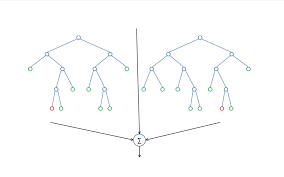
\includegraphics[scale=0.5]{figures/Chapter3AnnisaFathoroni1.png}
\caption{Random Forest}
\label{contoh}
\end{figure}

\end{itemize}

\item Cara Membaca Dataset

Berikut adalah cara membaca dataset :
\begin{itemize}
\item Buka Anaconda Navigator lalu jalankan Syder, kemudian import libraries yang dibutuhkan.
\item Masukkan kode python untuk membaca file csv, lalu jalankan

\begin{figure}[ht]
\centering
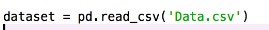
\includegraphics[scale=0.8]{figures/Chapter3AnnisaFathoroni5.jpeg}
\caption{Code Python}
\label{contoh}
\end{figure}

\item Maka pada window console akan menampilkan pesan berikut:

\begin{figure}[ht]
\centering
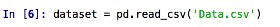
\includegraphics[scale=0.8]{figures/Chapter3AnnisaFathoroni6.jpeg}
\caption{Output}
\label{contoh}
\end{figure}

\item Dari explorer dapat terlihat dataset yang terimport.

\begin{figure}[ht]
\centering
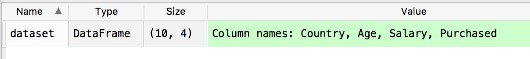
\includegraphics[scale=0.5]{figures/Chapter3AnnisaFathoroni7.jpeg}
\caption{Import Dataset}
\label{contoh}
\end{figure}

\item Lalu klik dataset cell, maka akan muncul seperti berikut :
\item Seperti yang terlihat pada gambar tersebut dataset ini memiliki Kolom Country, Age, dan Salary sebagai independent variable-nya dan kolom

\begin{figure}[ht]
\centering
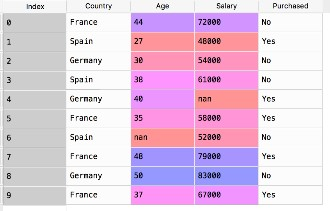
\includegraphics[scale=0.5]{figures/Chapter3AnnisaFathoroni8.jpeg}
\caption{Hasil Dataset Sel}
\label{contoh}
\end{figure}

\item Purchased sebagai dependent variable-nya.
\item Selanjutnya buat 2 matrix of features yang berisi values dari independent variable dan dependent variable.
\item Lalu tuliskan perintah berikut :

\begin{figure}[ht]
\centering
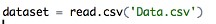
\includegraphics[scale=0.8]{figures/Chapter3AnnisaFathoroni9.jpeg}
\caption{Perintah}
\label{contoh}
\end{figure}

\item Perintah yang telah dibuat di atas akan membuat sebuah global environment baru dan muncul dataset.
\item Klik dataset tersebut maka muncul tabel berisi dataset.
\end{itemize}

\item Cross Validation

Cross-validation (CV) adalah metode statistik yang dapat digunakan untuk mengevaluasi kinerja model atau algoritma dimana data dipisahkan menjadi dua subset yaitu data proses pembelajaran dan data validasi / evaluasi. Model atau algoritma dilatih oleh subset pembelajaran dan divalidasi oleh subset validasi. Selanjutnya pemilihan jenis CV dapat didasarkan pada ukuran dataset. Biasanya CV K-fold digunakan karena dapat mengurangi waktu komputasi dengan tetap menjaga keakuratan estimasi.

\item Arti score 44\% pada random forest, 27\% pada decission tree dan 29\%dari SVM.

 Kalau maksud arti score 27\% pada decission tree adalah presentasi hasil dari perhitungan dataset, sedangkan maksud arti score 29\% dari SVM adalah hasil pendekatan jaringan saraf.  Hasil tersebut didapat dari hasil valdasi silang untuk memastikan bahwa membagi training test dengan cara yang berbeda. Sehingga didapat outputnya 44\% untuk hutan acak, 27\% untuk pohon keputusan, dan 29\% untuk SVM.

\item Confusion Matrix Dan Ilustrasinya
\begin{enumerate}
\item Perhitungan confusion matrix adalah sebagai berikut, akan saya beri contoh sederhana yaitu pengambilan keputusan untuk mendapatkan bantuan beasiswa. Saya menggunakan dua atribut, yaitu rekening listrik dan gaji. Ini adalah pohon keputusannya:
 
\begin{figure}[ht]
\centering
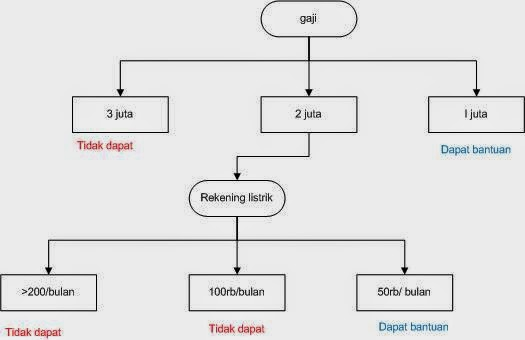
\includegraphics[scale=0.5]{figures/Chapter3AnnisaFathoroni2.jpg}
\caption{Pohon Keputusan}
\label{contoh}
\end{figure}
\end{enumerate}

Kemudian data testingnya adalah

\begin{figure}[ht]
\centering
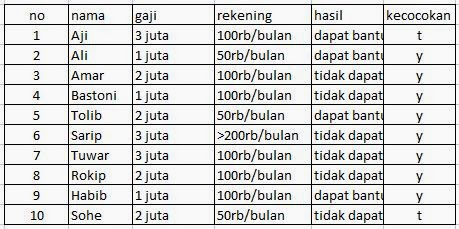
\includegraphics[scale=0.5]{figures/Chapter3AnnisaFathoroni3.jpg}
\caption{Data Testing}
\label{contoh}
\end{figure}

Yang pertama kita lakukan yaitu mencari 4 nilai yaitu a,b,c, dan d:

a= 5

b= 1

c= 1

d= 3

Kemudian kita dapat mencari nilai Recall, Precision, accuracy dan Error Rate

Recall =3/(1+3) = 0,75

Precision = 3/(1+3) = 0,75

Accuracy =(5+3)/(5+1+1+3) = 0,8

Error Rate =(1+1)/(5+1+1+3) = 0,2

\item Voting Random Forest Dan Ilustrasi Gambarnya.

\begin{itemize}
\item Pengertian Voting pada Random Forest

Metode ensemble dapat mencapai akurasi tinggi dengan membangun beberapa pengklasifikasi dan menjalankan masing-masing secara mandiri. Ketika classifier membuat keputusan, Anda dapat memanfaatkan yang terbaik keputusan umum dan rata-rata. Jika kita menggunakan metode yang paling umum, itu disebut voting

\item Ilustrasi Gambar Voting Random Forest :
\begin{figure}[ht]
\centering
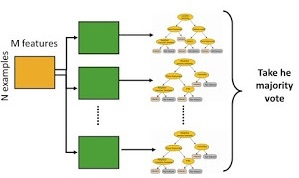
\includegraphics[scale=0.8]{figures/Chapter3AnnisaFathoroni4.jpg}
\caption{Voting Random Forest}
\label{contoh}
\end{figure}
\end{itemize}
\end{enumerate}